\documentclass[11pt]{article}
\usepackage{geometry}                
\geometry{letterpaper}                   

\usepackage{graphicx}
\usepackage{amssymb}
\usepackage{epstopdf}
\usepackage{float}
\usepackage[sort, numbers]{natbib}
\usepackage{url}
\setcitestyle{square}
\usepackage{amssymb, amsmath}
\DeclareGraphicsRule{.tif}{png}{.png}{`convert #1 `dirname #1`/`basename #1 .tif`.png}

%\title{Title}
%\author{Jo\"el Mathys, Marc Rauch}
%\date{date} 

\begin{document}



\thispagestyle{empty}

\begin{center}
\includegraphics[width=5cm]{ETHlogo.eps}

\bigskip


\bigskip


\bigskip


\LARGE{ 	Lecture with Computer Exercises:\\ }
\LARGE{ Modelling and Simulating Social Systems with MATLAB\\}

\bigskip

\bigskip

\small{Project Report}\\

\bigskip

\bigskip

\bigskip

\bigskip


\begin{tabular}{|c|}
\hline
\\
\textbf{\LARGE{Optimize Network Productivity}}\\
\textbf{\LARGE{by Simulating Ant Behaviour}}\\
\\
\hline
\end{tabular}
\bigskip

\bigskip

\bigskip

\LARGE{Jo\"el Mathys \& Marc Rauch}



\bigskip

\bigskip

\bigskip

\bigskip

\bigskip

\bigskip

\bigskip

\bigskip

Zurich\\
December 2017\\

\end{center}



\newpage

%%%%%%%%%%%%%%%%%%%%%%%%%%%%%%%%%%%%%%%%%%%%%%%%%

\newpage
\section*{Agreement for free-download}
\bigskip


\bigskip


\large We hereby agree to make our source code for this project freely available for download from the web pages of the SOMS chair. Furthermore, we assure that all source code is written by ourselves and is not violating any copyright restrictions.

\begin{center}

\bigskip


\bigskip


\begin{tabular}{@{}p{3.3cm}@{}p{6cm}@{}@{}p{6cm}@{}}
\begin{minipage}{3cm}

\end{minipage}
&
\begin{minipage}{6cm}
\vspace{2mm} \large Jo\"el Mathys

 \vspace{\baselineskip}

\end{minipage}
&
\begin{minipage}{6cm}

\large Marc Rauch 

\end{minipage}
\end{tabular}


\end{center}
\newpage

%%%%%%%%%%%%%%%%%%%%%%%%%%%%%%%%%%%%%%%



% IMPORTANT
% you MUST include the ETH declaration of originality here; it is available for download on the course website or at http://www.ethz.ch/faculty/exams/plagiarism/index_EN; it can be printed as pdf and should be filled out in handwriting


%%%%%%%%%% Table of content %%%%%%%%%%%%%%%%%

\tableofcontents

\newpage

%%%%%%%%%%%%%%%%%%%%%%%%%%%%%%%%%%%%%%%



\section{Abstract}
The amount of people transported by train in Switzerland has been constantly rising in the last years. This growth brings many questions to the SBB, the largest train company in Switzerland. \citep{SbbStats} In this paper we discuss the approach of maximizing the amount of people transported in the Swiss rail network. In an optimised scenario trains would be able to fill their capacity and more people could be transported with the same resources. This increase of efficiency of the trains would help with counteracting the pressure on the rail network. 
We will discuss this problem with a model, which is inspired by the path finding of ant colonies. Ants have been found to be very efficient at finding paths, which lead to food sources. Those paths are optimised in terms of travel time to the source and the quality of the food.

\section{Individual contributions}
The paper is an team effort of Jo\"el Mathys and Marc Rauch. There was no strict division of the work, but both of us had a focus on a certain part of the paper.
\begin{itemize}
  \item Jo\"el Mathys: Simulation, visualisation, graph generation, writing of report
  \item Marc Rauch: Behaviour of single ants, writing of report
\end{itemize}



\section{Introduction and Motivations} \label{intro}
The amount of people who use the Swiss rail network has risen by over 900\% in the last 100 years. However the number of train stations and the total distance covered by rails have only seen a growth of less then 20\% \citep{SbbStats}. Therefore the efficiency, of transporting those customers has become more important. In this paper we describe the efficiency as passengers transported per time. The goal is to maximize this efficiency and transport as many passengers as possible in a given time period. For this optimization the resources should only be redistributed, but no additional trains or stations have to be added to the system. 
We assume, that the most efficient way to transport these people is a compromise between distance to the destination and the size of the target city. If the train connection is over a long distance, then the destination city has to be large, so that enough passengers have the desire to use that connection. If the distance is short, and the demand for the connection is lower, it is still worthwhile to allocate some resources to that connection.
Ants have a similar goal when searching for a new food source. They have to find a compromise between distance to a source and the quality of the provided food. Many studies show, that the method used by ants to find that optimum is very efficient. In fact they are so efficient, that over the last 20 years lots of research was done in solving problems with the inspiration from ants. These so called ant colony optimization (ACO) algorithms are mainly used in solving hard problems, which can not be efficiently solved. Through the research many promising algorithms have been found \citep{Aco1}.
In the rest of this paper we are going to explore the following questions:
\begin{itemize}
  \item How can the productivity in a network be maximised?
  \item What does this imply on the Swiss rail network?
\end{itemize}
We are going to investigate those questions with the help of an ACO. The analogy between the ant model and the rail system will be described In chapter \ref{relationNetwork}. The productivity in the ant network is defined as the amount of food, that is brought back to the colonies per time. We are looking to investigating the following parameters:
\begin{enumerate}
	\item The population sizes do not change.
	\item The ants are free to change colonies globally.
	\item The ants can only change colonies locally.
\end{enumerate}
In the end we compare the resulting efficiency of each of those strategies. 


\section{Description of the Model} \label{modeldesc}
The model is based on research on the ant Lasius niger, in the book "Self-organization in biological systems" \citep{camazine2003}. This paper describes the process of trail formation in ants. This phenomenon can easily observed in the wild, by placing some sugar solution. After a short while the food will be discovered and shortly after, the number of ants at the food source will increase rapidly, until eventually it stabilizes and a well established trail of ants can be observed from the nest to the sugar. To study this behaviour, several experiments have been conducted on a colony of Lasius niger. The research was done under Laboratory conditions, so that the terrain could be controlled and therefore the experiments are repeatable. The terrain was constructed in such a way, that there was one path leading away from the colony, which then split into two paths with a food source at the end of both paths. The length, as well as the quality of the food sources could be controlled. Then the behaviour of the ants was observed and formulated as a mathematical model.
\subsection{Trail laying}
 It was found, that the ants would place chemicals, so called pheromones, which motivates other ants to follow the laid path. When an ant finds a food source it will lay pheromones on the way back to the nest and on the following trips to the source. This acts as a positive feedback for the other ants, which are likely to follow that trail. Trail laying is only observed by ants, who found food. The intensity of the laid trails is dependant on the quality of the found food. The better the food source, the more pheromones will be deposited. The frequency of laying pheromones is also reduced based on the current direction of the ant. If the ant is walking in a trajectory with a bad angle to the direct route to the nest less pheromones will be placed. The placed chemicals also evaporate over time. They undergo an exponential decay given by formula \ref{pheromone1}.
 \begin{equation} \label{pheromone1}
  \frac{dC}{dt}=-\frac{1}{l}C
 \end{equation}
 where l is the lifetime of the pheromones and C the concentration.
 \subsection{Binary choices}
 In the experiment there was a choice the ants had to make, when the path split into two and they have to decide, whether to go left or right. This decision is made based on the concentration of pheromones on each branch. So that the branch with a higher concentration of pheromones on it has a better chance of being chosen. For that decision a formula for the probability of choosing one of the two branches was found.
  \begin{equation} \label{binaryChoice}
 P_L = \frac{(k+C_L)^n}{(k+C_L)^n+(k+C_R)^n} \ and \  P_R = 1-P_L
 \end{equation}
 n is the non-linearity factor. with a high value of n a branch with little more pheromones then the other will be strongly favoured. With experiments it is approximately found that $n=2$. k stands for the likelihood of the ant taking a path with no pheromones on it. P is the probability of choosing the left or right path and C the concentration of pheromones on each path. 
 \subsection{U-Turns}
 It is often observed, that ants on a trail make an U-turn, return to the last branch point and follow the other path. After an U-turn the ant does not lay a trail, until it has gone back to the branch and follows the new path. There are two causes of this behaviour. If the amount of pheromones on the trail is low the ant may turn around. The second reason is direction based. If the orientation to the target is not good the probability of an U-turn is high. This probability can be modelled by equation \ref{UTurn}. \citep{camazine2003}
\begin{equation} \label{UTurn}
 P=\frac{P_0}{1+\alpha C}
\end{equation}

$P_0$ stands for the probability of an direction based U-turn. $\alpha$ describes the importance of the pheromone based U-turn.
\subsection{Extensions}
 For our project we could not use the model as given in the paper, So the model was changed in some aspects to ease the implementation and add additional functionality. Because the goal of this paper is to model more complicated networks then the one with only one binary decision, formula \ref{binaryChoice} has to be adapted to support a choice between more than just two paths. 
\begin{equation} \label{multiDecisions}
P_i = \frac{(k+C_i)^n}{\sum{_{j=1}^{nr}(k+C_j)^n}}
\end{equation}  
 nr describes the number of adjacent edges on the node.
\begin{figure}[H]
	\centering
	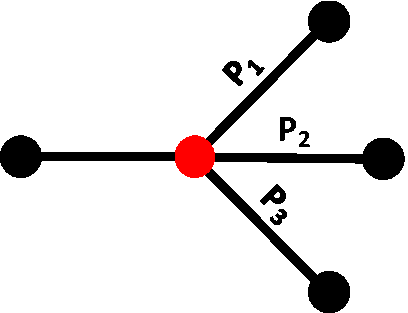
\includegraphics[scale=0.5]{decision3.pdf}
	\caption{Decision of an ant approaching a traffic node of degree 4 (represented in red) from the left hand side, with the probabilities $P_1$ to $P_3$ of the next edge.}
\end{figure}
Notice, that although the graph is not directed the decision of taking the same edge back to where the ant came from is not allowed. This edge is not part of the decision set.
Because we represent the terrain on which the ants move by a graph, the implementation of direction based turns is very difficult. Therefore we set $P_0 = 1$ in equation \ref{UTurn} and are left with the pheromone based U-turn equation.
\subsection{Relation to the Swiss rail network}\label{relationNetwork}
The Swiss rail network should be described with the help of this model. The network is given as a graph, which connects all train station to each other. The following analogies between the ant and the train model have been made:
\begin{itemize}
  \item The train stations represent the sources, as well as the colonies.
  \item The ants are replaced by trains.
  \item The food is represented by the travelling passengers.
\end{itemize}
 In the new model the train stations are the starting point and the destination of all trains. Therefore there is no more distinction between colonies and sources, since colonies are sources for ants of a different colony. When a train reaches its destination, it gets filled up with people. The more people are at that station the more passengers will board the train. The amount of waiting passengers at the station is equivalent to the quality of the food. With every arrival of trains at a station the quality of this station decreases, as there are less passengers waiting to be transported. This devaluation of the stations is counteracted by a regeneration rate, which is proportional to the popularity of the station. A popular station has a high regeneration rate, as there are lots of new potential passengers arriving in a given time step. With those analogies the productivity, which was defined as food carried to each colony per time is defined as people transported to each station per time. This is exactly the quantity, which we want to optimize.

\section{Implementation}
\input{implementation}

\section{Simulation Results and Discussion}

\section{Summary and Outlook}

\begin{flushleft}
\nocite{*}
\bibliography{References}
\bibliographystyle{apalike}
\end{flushleft}


\end{document}  



 
